\documentclass{article}
\usepackage[utf8x]{inputenc}
\usepackage{amsmath}
\usepackage{MathUnicode}
\usepackage{upquote,textcomp}
\usepackage[a4paper,bindingoffset=0.2in,left=1in,right=1in,top=1in,bottom=1in,footskip=.25in]{geometry}

\usepackage{changepage}

\usepackage[spanish]{babel}
\usepackage{tabularx}
\usepackage{multirow}
\usepackage{graphicx}
\usepackage{listings}
\usepackage[font=scriptsize]{caption}
\usepackage[font=scriptsize]{subcaption}
\usepackage{caption}
\usepackage[yyyymmdd,hhmmss]{datetime}
\usepackage{color}

\usepackage[colorlinks,urlcolor=blue]{hyperref}
\usepackage{xifthen}

\newcounter{problem}
\newcounter{solution}
\renewcommand{\theenumi}{\alph{enumi}}

\newcommand\Problem[1][]{%
  \color{blue}
  \stepcounter{problem}%
  \ifthenelse{\isempty{#1}}{\textbf{Problema \theproblem.}}{\textbf{Problema #1.}}

  \setcounter{solution}{0}%
}

\newcommand\TheSolution{%
  \color{black}
  \textbf{Solución:}\\%
}

\newcommand\ASolution{%
  \stepcounter{solution}%
  \textbf{Solución \thesolution:}\\%
}


\setlength{\arrayrulewidth}{1mm}
\setlength{\tabcolsep}{18pt}
\renewcommand{\arraystretch}{1.5}


\author{Pedro Valero Mejía}
\title{Ejercicios de Sistemas Informáticos II}
\parindent 0in
\parskip 1em

\begin{document}

\maketitle
%%%%%%%%%%%%%%%%%%%%%%%%%%%%%%%%%%%%%%%%%%%%%%%%%%%%%%%%%%%%%%%%%%%%%%%%%% PROBLEMA 1
\Problem[1]
Los mensajes llegan a un servidor de descifrado de manera poissoniana con un ritmo medio de llegada de 360 mensajes por minuto. Los tiempos de descifrado son proporcionales a la longitud de los mensajes, los cuales se distribuyen aproximadamente de forma exponencial, con una longitud media de 1500 bytes. La velocidad del servidor de descifrado es de 10Kbyte/s. ¿Cuál es el tiempo medio de espera de respuesta por mensaje? ¿Cuál es el número medio de mensajes en el sistema de descifrado?

\TheSolution

El número de mensajes por unidad de tiempo es la tasa de llegadas, que deberemos escribir en unidades del Sistema Internacional:
\[λ = 360 min^{-1}=6 s^{-1}\]

Por otro lado tenemos que si la longitud del mensaje es una variable aleatoria que sigue una distribución exponencial y el tiempo de procesamiento es proporcional a la longitud, el tiempo de servicio será una variable aleatoria exponencial de media:
\[T_s = \frac{1500 bytes}{10000 bytes/s} = \boxed{0.15s}\]

A partir de aquí podemos calcular la tasa de servicio:
\[μ = \frac{1}{T_s} = 6.66 s^{-1}\]

Se trata de un sistema M/M/1 de modo que podemos calcular el número medio de mensajes en el sistema a partir, únicamente, del factor de utilización según la fórmula:
\[L=\frac{ρ}{1-ρ}=\frac{λ/μ}{1-λ/μ}=\frac{λ/μ}{(μ-λ)/μ}=\frac{λ}{μ-λ}=\boxed{9.09}\]


%%%%%%%%%%%%%%%%%%%%%%%%%%%%%%%%%%%%%%%%%%%%%%%%%%%%%%%%%%%%%%%%%%%%%%%%%% PROBLEMA 2

\Problem
Se tiene un servidor en Internet que recibe un tráfico de Poisson a un ritmo medio P peticiones/s. El tiempo que tarda en atender una petición se encuentra distribuido exponencialmente, siendo capaz de procesar S peticiones/s.

Debido al éxito del servidor, a los quince días de su aparición en Internet su tráfico se ha multiplicado por un factor K. Para resolver el problema, se cambia de ordenador, solicitando uno de potencia K veces superior al actual.

Calcular el nuevo número medio de clientes en el sistema servidor, y el nuevo tiempo de permanencia en el sistema tras la ampliación del servidor en función de los valores anteriores al cambio.

\newpage
\TheSolution

Tras el éxito del servidor pasamos a tener una tasa de llegadas:
\[λ = K \cdot P\]

Al cambiar la potencia del ordenador multiplicándola por $K$ estamos reduciendo el tiempo de servicio según ese mismo factor y multiplicando la tasa de servicio por $K$:
\[μ = S \cdot K\]

Se trata de un sistema M/M/1 donde el número de clientes en el sistema sólo depende del factor de utilización del mismo que, en este caso, no ha cambiado.

Por tanto seguimos teniendo el mismo número medio de clientes en el sistema que antes de producirse los cambios.

Para calcular el nuevo tiempo de permanencia nos apoyamos en el Teorema de Little que nos permite escribir
\[W = \frac{L}{λ}\]
puesto que $L$ no ha cambiado y λ se ha hecho $K$ veces mayor, el tiempo medio de permanencia en el sistema se ha reducido en un factor de $K$.

%%%%%%%%%%%%%%%%%%%%%%%%%%%%%%%%%%%%%%%%%%%%%%%%%%%%%%%%%%%%%%%%%%%%%%%%%% PROBLEMA 3

\Problem
Se desea diseñar un servidor para satisfacer un tráfico de Poisson con un tiempo medio entre peticiones de 10 s. El servicio a proporcionar tiene una duración distribuida exponencialmente con media de 16 s. Calcular:
\begin{enumerate}
\item El número mínimo de servidores para satisfacer el tráfico requerido.
\item Con dicho número de servidores, el tiempo medio de espera en cola por petición.
\item El tiempo medio de espera en cola, en caso de independizar cada servidores, asignándole una cola de espera a cada uno de ellos, y repartiendo el tráfico entre ellos de modo aleatorio para que cada uno reciba la mitad del total.
\end{enumerate}

\TheSolution

\begin{enumerate}
\item

Si nos llega una petición cada 10 segundos, tenemos una tasa de llegadas de
\[λ = 0.1 s^{-1}\]

Dado que el tiempo medio de servicio es de 16s y tenemos $c$ servidores, la tasa de servicio es:
\[μ=\frac{0.0625}{c}\]

Si queremos que el sistema no colapse, necesitamos que el factor de utilización sea menor que 1, es decir:
\[ρ = \frac{λ}{cμ}<1 \implies λ < cμ \implies c>1.6\]
necesitamos $\boxed{2}$ servidores para satisfacer el tráfico requerido
\item

Para este ejercicio nos apoyamos fuertemente en el formulario. Nos encontramos ante un sistema M/M/2 y para calcular el tiempo de espera en cola debemos calcular el número de clientes en el sistema con ayuda de las fórmulas. Una vez obtenido este valor aplicamos el Teorema de Little para calcular el tiempo medio de estancia en el sistema y le restamos el tiempo medio de servicio.

Vamos a ello:

\[ρ = \frac{λ}{2\cdot μ}=0.8\]

\[p_0 = \left[ \sum_{n=0}^{c-1}\frac{(λ/μ)^n}{n!}+\frac{(λ/μ)^c}{c!(1-ρ)}\right]^{-1}=\left[1+1.6+\frac{2.56}{0.4}\right]^{-1}=(9)^{-1}=0.11\]

\[p_2=p_0\frac{c^c}{c!}\left( \frac{λ}{cμ}\right)^n=0.11\cdot 2 \cdot 0.64 = 0.14\]
\[P_q=\frac{p_c}{1-ρ}=0.71\]

Finalmente
\[L=\frac{P_q ρ}{1-ρ}+cρ=4.44\]

Aplicando Little nos queda
\[W = \frac{L}{λ}=44.4\]

Puesto que el tiempo de servicio es de 8s, el tiempo medio de espera en cola asciende a
\[W-T_s=\boxed{36.4s}\]
\item

Este caso es equivalente al ejercicio anterior con $K=0.5$ por lo que tenemos
\[W_n =\frac{W_o}{K}=88.8s\]

lo que implica
\[W-T_s = \boxed{56.8s}\]
\end{enumerate}

%%%%%%%%%%%%%%%%%%%%%%%%%%%%%%%%%%%%%%%%%%%%%%%%%%%%%%%%%%%%%%%%%%%%%%%%%% PROBLEMA 4

\Problem
Se quiere diseñar un servidor de emisión de certificados en Internet para que sea capaz de atender una media de 10 peticiones por segundo con un tiempo medio de respuesta de 0.1s. Sabiendo que el programa de generación del certificado es siempre el mismo, independientemente del cliente, y requiere la ejecución de 10.000 instrucciones de código máquina, calcular la potencia de ordenador (en MIPS) necesaria para su ejecución,
suponiendo despreciable cualquier otra carga en el mismo.

\TheSolution

Queremos ejecutar 10.000 instrucciones de código en 0.1s deberemos tener una potencia de \boxed{0.1 MIPS}


%%%%%%%%%%%%%%%%%%%%%%%%%%%%%%%%%%%%%%%%%%%%%%%%%%%%%%%%%%%%%%%%%%%%%%%%%% PROBLEMA 5

\Problem
Una fracción p del tráfico de salida procedente de un servidor con tiempo de servicio distribuido exponencialmente con media Ts se realimenta a su entrada. El tráfico nuevo llega al servidor con un ritmo medio R. Calcular el factor de utilización del servidor y el tiempo medio de estancia en el
sistema.

\TheSolution

Empezamos calculando la tasa de llegadas:
\[λ = R + pλ \implies λ = \frac{R}{1-p}\]

La taasa de servicio es
\[μ= \frac{1}{T_s}\]

Así el factor de utilización sería
\[ρ=\frac{λ}{μ}=\boxed{\frac{R \cdot T_s}{1-p}}\]

Sabiendo que es un sistema M/M/1 podemos calcular el número medio de clientes en el sistema como:
\[L = \frac{ρ}{1-ρ}=\frac{R\cdot T_s}{1-p-R\cdot T_s}\]

Aplicando ahora el Teorema de Little podemos calcular el tiempo medio de estancia en el servidor como:
\[W = \frac{L}{λ}=\boxed{\frac{T_s}{(1-p-R\cdot T_s)(1-p)}}\]

%%%%%%%%%%%%%%%%%%%%%%%%%%%%%%%%%%%%%%%%%%%%%%%%%%%%%%%%%%%%%%%%%%%%%%%%%% PROBLEMA 6

\Problem
En una determinada red de área local se dispone de un servidor de comunicaciones, que actúa como encaminador de mensajes de aplicación entre la dicha red y una red remota, a la que se encuentra conectado a través de una línea dedicada de velocidad $2\cdot 10^6$ bps.

A la red de área local hay conectados un número muy grande de terminales clientes, que envían mensajes cuyo tamaño se encuentra distribuido exponencialmente con un valor medio de 1 KByte.

Se puede considerar que los mensajes llegan al servidor siguiendo un ritmo de Poisson. Se pide:
\begin{enumerate}
\item Si el servidor de comunicaciones recibe un promedio de 180 peticiones/s, calcular tiempo medio que transcurre desde que un mensaje es recibido en el servidor hasta que llega al punto destino.
\item Calcular el número máximo de peticiones por segundo que se estarán procesando si se sabe que el tamaño medio de memoria que ocupa la cola de mensajes en espera de ser procesados es de 10 KBytes.
\end{enumerate}

\TheSolution

En este ejercicio el tiempo de procesamiento de mensaje por parte del servidor es el tiempo que tarda dicho servidor en enviar el mensaje a través del enlace descrito.

\begin{enumerate}
\item
Tenemos una tasa de peticiones
\[λ = 180 s^{-1}\]

Sabiendo el tamaño medio de los mensajes y la capacidad de transmisión de la línea dedicada, podemos calcular el tiempo de servicio
\[T_s = \text{tamaño}/\text{velocidad} = 0.0041s\]

lo que nos da una tasa de servicio de
\[μ=\frac{1}{T_s}=244.14 s^{-1}\]

A partir de aquí podemos calcular el factor de utilización del sistema
\[ρ = \frac{λ}{μ}=0.74\]

y, puesto que estamos ante un sistema M/M/1 podemos calcular el número medio de clientes en el sistema como
\[L = \frac{ρ}{1-ρ}=2.85\]
y a partir del Teorema de Little calculamos el tiempo medio de estancia en el sistema, que es el dato pedido
\[W= \frac{L}{λ}= \boxed{0.016s}\]

\item

Ahora nos encontraríamos ante un sistema M/M/1/K siendo $K$ el número máximo de clientes en el sistema que se calcula como el número máximo de clientes en cola +1 (el que se está procesando).

Puesto que conocemos el tamaño de la cola y el tamaño de los mensajes, podemos calcular $K=10$ mensajes. Es decir, tenemos un sistema M/M/1/10 y nos piden calcular $L$, el número máximo de clientes en el sistema.

Los valores de λ y μ calculados en el apartado anterior siguen siendo válidos, pues no han cambiado las condiciones de llegada y procesamiento de mensajes.

Procedemos pues a calcular $L$:
\[L = \frac{λ/μ}{1-λ/μ}\frac{1-(K+1)(λ/μ)^K+K(λ/μ)^{K+1}}{1-(λ/μ)^{K+1}}=\frac{λ/μ}{1-λ/μ}\frac{1-(3)(λ/μ)^2+2(λ/μ)^{3}}{1-(λ/μ)^{3}}=\]
\[=\frac{0.74}{0.26}\frac{0.17}{0.6}=\boxed{0.81}\]

\end{enumerate}
%%%%%%%%%%%%%%%%%%%%%%%%%%%%%%%%%%%%%%%%%%%%%%%%%%%%%%%%%%%%%%%%%%%%%%%%%% PROBLEMA 7

\Problem
Deseamos instalar un servidor de envío de mensajes ("busca") a una serie de abonados. El número de abonados, que suponemos muy grande, envía mensajes a nuestro servidor, desde donde se envían a su destino mediante un sistema de transmisión por radio. Los mensajes llegan según un proceso de Poisson con una tasa de llegadas L. El tiempo de servicio (total del proceso y envío del mensaje) se puede considerar distribuido exponencialmente con valor medio S. El esquema de bloques del servicio es el siguiente:

\begin{center}
  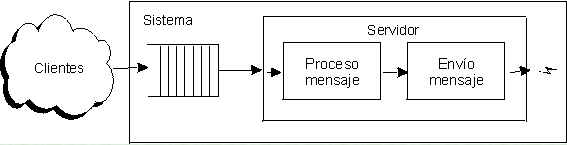
\includegraphics[keepaspectratio=true,width=\linewidth]{img/ej7.png}
\end{center}


\begin{enumerate}
\item Calcular el tiempo medio que transcurre desde que un mensaje llega al sistema hasta que es servido a su destino.
\item La tarifa del servicio es de P Euros por mensaje transmitido, pero se proporciona un descuento de D Euros por cada segundo que el mensaje tarde en llegar a su destino. Calcular los ingresos medios esperados por mensaje transmitido.
\item Calcular a partir de qué tasa de peticiones el tiempo de espera será tal que el mensaje se deba transmitir gratuitamente (se supone que nunca se aplica un descuento mayor que el coste de transmisión del mensaje).

\end{enumerate}

\newpage
\TheSolution

\begin{enumerate}
\item
Tenemos las tasas de llegadas y servicio
\[λ=L \ \ \ μ=\frac{1}{S}\]

A partir de estos datos calculamos el factor de utilización
\[ρ = \frac{λ}{μ}=L\cdot S\]

Puesto que nos encontramos ante un sistema M/M/1 podemos calcular el número de clientes en el sistema a partir del factor de utilización:
\[L_c=\frac{ρ}{1-ρ}=\frac{L}{S-L}\]

Por último calculamos el tiempo medio de estancia en el sistema a partir del teorema de Little:
\[W = \frac{L_c}{λ}=\frac{L\cdot S}{S-L_c}\]

\item

Los ingresos medios serán el precio por mensaje por el número medio de mensajes que se manipulan menos el dinero que se devuelve por segundo de retraso multiplicado por el retraso habitual de procesamiento de los mensajes.

Nos queda la fórmula
\[\text{Ingresos} = P \cdot L_c - D \cdot W\]

\item

Basta con igualar los ingresos a 0:
\[P\cdot L_c = D \cdot W \iff P \cdot L_c = \frac{L\cdot S}{S-L_c} \]
Ahora simplemente despejamos $L_c$ y a partir de ahí despejamos ρ que usaremos para calcular λ.

\end{enumerate}

%%%%%%%%%%%%%%%%%%%%%%%%%%%%%%%%%%%%%%%%%%%%%%%%%%%%%%%%%%%%%%%%%%%%%%%%%% PROBLEMA 8

\Problem
Una red de una entidad financiera consta de una serie de terminales remotos, en número que podemos considerar muy grande, conectados mediante líneas telefónicas alquiladas full duplex a un multiplexor de terminales. Dicho multiplexor entrega los mensajes recibidos a un servidor, que ejecuta los programas transaccionales necesarios para atender al mensaje recibido, y devuelve los resultados al cliente a través del mismo multiplexor. El esquema de bloques del servicio es el siguiente:

\begin{center}
  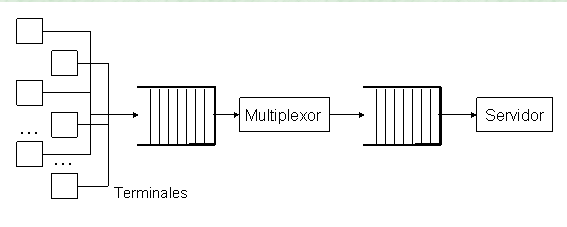
\includegraphics[keepaspectratio=true,width=\linewidth]{img/ej8.png}
\end{center}

Los mensajes de las oficinas llegan al multiplexor según un proceso de Poisson con una tasa de llegadas total de 3 s -1 (es decir, incluyendo las peticiones de todos los servidores) y su longitud media es de 1 Kbyte. El tiempo de servicio del multiplexor por mensaje (total del proceso y envío del mensaje) se puede considerar distribuido exponencialmente con valor medio 250 ms.

\begin{enumerate}
\item Calcular la ocupación media en memoria de la cola de mensajes en espera de servicio del multiplexor
\item Calcular la tasa de llegadas al servidor.
\item Los mensajes que llegan al servidor son de tres tipos básicos. El tiempo de proceso en el servidor depende del tipo de mensaje recibido, de acuerdo a la siguiente tabla:

\begin{center}
\begin{tabular}{| c | c | c |}
\hline
  \textbf{Identificador mensaje} &  \textbf{Probabilidad} & \textbf{Tiempo de proceso}\\
\hline
0 & 0.5 & 0.1 \\
1 & 0.3 & 0.2 \\
2 & 0.2 & 0.4 \\
\hline
\end{tabular}
\end{center}

Estos tiempos incluyen lo que tarda el mensaje de respuesta en llegar al terminal remoto. Esta transmisión del mensaje de respuesta se supone que no afecta al tiempo de proceso del multiplexor ni a la comunicación por la línea que lo une con el terminal.

Calcular el tiempo medio de estancia en el servidor de las solicitudes.


\end{enumerate}

\TheSolution

\begin{enumerate}

\item

Tenemos una tasa de llegadas $λ=3$ y un tiempo de servicio por parte del multiplexor de 250ms lo que nos da una tasa de servicio $μ=4$.

Analizando por separado el multiplexor, tenemos un sistema M/M/1 de modo que calculamos ρ y lo usamos para calcular el número medio de clientes $L$.

\[π=\frac{λ}{μ}=0.75\]
\[L=\frac{ρ}{1-ρ}=3\]

\item

La tasa de llegadas al servidor es exactamente la misma que la tasa de llegadas al multiplexor. Cada mensaje que llega a este último es enviado al servidor

\item

El tiempo de servicio en el servidor se puede calcular como una suma ponderada de los tiempos de servicio de cada tipo de mensaje.
\[T_s = 0.5\cdot 0.1+0.3\cdot 0.2+0.2\cdot 0.4=0.19 \implies μ = \frac{1}{T_s}=5.26\]

Volvemos a tener un sistema M/M/1. Calculamos ρ, a partir de ahí $L$ y por último empleamos el Teorema de Little para calcular el tiempo medio de estancia en el sistema.

\[ρ = \frac{λ}{μ}=0.57 \implies L=\frac{ρ}{1-ρ}=1.33 \implies W = \frac{L}{λ}=0.44 s\]
\end{enumerate}

\newpage
%%%%%%%%%%%%%%%%%%%%%%%%%%%%%%%%%%%%%%%%%%%%%%%%%%%%%%%%%%%%%%%%%%%%%%%%%% PROBLEMA 9

\Problem
El servidor de fecha y hora de una red resuelve cada petición en un tiempo que se puede suponer distribuido exponencialmente con media 100 ms. La red se compone de un número muy grande de clientes que realizan peticiones, cuya llegada al servidor se considera que sigue un proceso de Poisson.
\begin{enumerate}
\item Calcular el número máximo de peticiones por segundo que se podrán satisfacer para obtener un tiempo medio de respuesta del servidor menor o igual que 1 s.
\item Calcular el tiempo medio de servicio necesario para poder satisfacer el doble de peticiones reduciendo el tiempo de respuesta a la mitad.

\end{enumerate}

\TheSolution

\begin{enumerate}
\item Nos piden calcular el número máximo de peticiones por segundo que se pueden satisfacer, es decir, tenemos que calcular λ.

Sabemos que el tiempo medio de servicio es de 100 ms, por lo que tendremos que
\[μ = \frac{1}{T_s}=\frac{1}{100 ms} = \frac{1}{0.1s}=10s^{-1}\]

El tiempo de servicio es el tiempo medio de estancia en el sistem y queremos que sea menor que 1, por lo que:
\[W=\frac{L}{λ}=\frac{\rho}{λ(1-\rho)}=\frac{1}{μ-λ} < 1 \implies μ > λ +1\]
por lo que el sistema no podrá atender más de 9 peticiones por segundo.

\item Ahora queremos que λ=18 manteniendo el tiempo medio de respuesta de 1 s. Sustituyendo en la ecuación anterior tenemos:

\[W < \frac{1}{2} \implies μ > λ +2 \implies μ > 20 \implies T_s < \frac{1}{20} = 50 ms\]
\end{enumerate}

%%%%%%%%%%%%%%%%%%%%%%%%%%%%%%%%%%%%%%%%%%%%%%%%%%%%%%%%%%%%%%%%%%%%%%%%%% PROBLEMA 10

\Problem
Un servidor web de aplicaciones se compone de los siguientes elementos

\begin{center}
  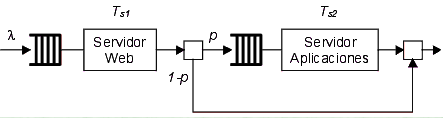
\includegraphics[keepaspectratio=true,width=\linewidth]{img/ej10.png}
\end{center}

La llegada de solicitudes al sistema se puede considerar como un proceso de Poisson, con una tasa de llegadas de 6 peticiones por segundo. Existe un número muy grande de clientes, de modo que el número de peticiones pendientes de servicio no afecta al ritmo de llegada de nuevas peticiones.

El servidor Web atiende las peticiones de páginas estáticas e imágenes, empleando para ello un tiempo que se puede considerar distribuido exponencialmente con un valor medio de 50 ms. Se considera que el servidor procesa las peticiones de modo iterativo, es decir, de una en una.

Un 10\% de las peticiones procesadas por el servidor web requieren que, adicionalmente al proceso realizado por dicho servidor, se ejecute un programa externo. Esta ejecución se realiza en un servidor de aplicaciones, cuyo tiempo de servicio también se puede considerar distribuido exponencialmente con un valor medio de 1 s. También en este caso se considera que el servidor procesa las peticiones de modo iterativo.

\begin{enumerate}
\item Calcular el tiempo medio de estancia en el sistema de las peticiones que atiende únicamente el servidor Web, justificando el modelo de cálculo elegido.

\item Calcular el tiempo medio de estancia en el sistema de las peticiones que necesitan ser atendidas por ambos servidores, justificando el modelo de cálculo elegido.

\item Calcular el tiempo medio de estancia en el sistema total.

\item Realizando medidas sobre el sistema en producción se descubre que el tiempo de servicio del servidor web no sigue una distribución exponencial, sino una distribución cuyo coeficiente cuadrático de variación es igual a 5. Justificar la validez o invalidez del modelo empleado en los apartados anteriores, indicando las alternativas si no se considera válido.
\end{enumerate}

\TheSolution

\begin{enumerate}
\item
Para esta parte podemos suponer que el sistema se acaba al salir del servidor de modo que nos encontramos ante un sistema M/M/1 bastante sencillo. Vamos a calcular el tiempo medio de estancia en ese sitema reducido como hacemos siempre.

\[λ = 6, T_s = 50 ms \implies μ=\frac{1}{T_s}=20 \implies ρ = \frac{λ}{μ}=0.3\]

\[L=\frac{ρ}{1-ρ}=0.43 \implies W = \frac{L}{λ}=0.07s\]

\item

Puesto que no tenemos retroalimentación, la tasa de llegadas a este segundo sistema sería del 10\% de la tasa de llegadas al Servidor Web. Calculamos este nuevo λ y repetimos los cálculos del apartado anterior.

\[λ = 0.1\cdot 6 = 0.6, T_s = 1 s \implies μ=\frac{1}{T_s}=1 \implies ρ = \frac{λ}{μ}=0.6\]

\[L=\frac{ρ}{1-ρ}=1.5 \implies W = \frac{L}{λ}=15s\]

\item

\[W = W_{s_1}+p\cdot W_{s_2} = 1.57s\]

\item

El modelo empleado no será válido ya que para serlo el coeficiente cuadrátido de variación debería ser muy próximo a 1, cosa que no se cumple.

A fin de ajustar las estimaciones deberíamos repetir los cálculos considerando una distribución de tipo hiperexponencial

\end{enumerate}


%%%%%%%%%%%%%%%%%%%%%%%%%%%%%%%%%%%%%%%%%%%%%%%%%%%%%%%%%%%%%%%%%%%%%%%%%% PROBLEMA 11

\Problem Un middleware orientado a colas de mensajes (MOM) recibe mensajes en una cola local de todos los ordenadores que componen la red de modo aleatorio. La llegada de mensajes al MOM se puede considerar como un proceso de Poisson, con una tasa de llegadas de 10 peticiones por segundo. Existe un número muy grande de clientes, de modo que el número de peticiones pendientes de servicio no afecta al ritmo de llegada de nuevas peticiones. La longitud de los mensajes que se recibe es de 25Kbytes. El tamaño disponible para almacenar mensajes en la cola se supone ilimitado. Los mensajes recibidos en esta cola son procesados por dos servidores. El tiempo de servicio en cualquiera de ellos se puede considerar distribuido exponencialmente con un valor medio de 50 ms. Tan pronto como uno de los servidores esté libre, tomará el primer mensaje de la cola y lo procesará sin interrupciones.
\begin{enumerate}
\item Calcular el tamaño medio, en Kbytes, que tendrá la cola de mensajes en el MOM.
\item Calcular el tiempo medio de estancia en el sistema de las peticiones de los clientes.
\item Calcular cuál es la probabilidad de que el tamaño de la cola de mensajes sea mayor de 100 Kbytes.
\end{enumerate}

\TheSolution

Los datos que podemos extraer del enunciado son:
\[\left\{
\begin{array}{l}
λ = 10 \\
\text{Longitud de mensaje } 25Kb \\
\text{Colas infinitas} \\
\text{2 servidores con tiempo de servicio exponencial} \\
T_s = 50ms
\end{array}
\right.\]

Antes de hacer ningún cálculo, reconocemos que se trata de un modelo M/M/2
\begin{enumerate}
\item
Para calcular el tamaño medio de la cola de mensajes basta con calcular el número medio de mensajes en la cola y multiplicarlo por el tamaño de cada mensaje.

Por el teorema de Little tenemos

\[L_q = λ W_q\]

Pero sabemos que el tiempo de estancia en el sistema es la suma del tiempo de servicio más el tiempo de espera en cola, de modo que
\[L_q = λ w_q = λ (W-T_s)\]

y aplicando nuevamente el teorema de Little para calcula W tenemos:
\[L_q = λ\left(\frac{L}{λ}-\frac{1}{μ}\right)=L-cρ\]

Empezamos calculando el factor de utilización del sistema:
\[ρ = \frac{λ}{2μ}=\frac{λT_s}{2}=10\cdot 25ms = 0.25\]

Calculemos ahora el número medio de unidades en el sistema:
\[L=\frac{P_qρ}{1-ρ}+cρ\]
pero antes necesitamos conocer $P_q$:

\[P_q = \frac{p_c}{1-ρ}\]
y para ello necesitamos $p_c$ siendo $c=2$.

Para calcular $p_2$ tenemos que emplear la fórmula:
\[p_2=p_0\frac{c^c}{c!} \left(\frac{λ}{cμ}\right)^n\]

para lo que necesitamos conocer $p_0$.

\[p_0 = \left(1+0.5+\frac{0.5^2}{2\cdot 0.75}\footnote{Puesto que ρ < 1}\right)^{-1} = \frac{1}{1.64}=0.6\]

Una vez tenemos esto podemos calcular $p_2$.
\[p_2=p_0\frac{c^c}{c!} \left(\frac{λ}{cμ}\right)^n=0.6\cdot \frac{4}{2}\cdot (0.25)^2 = 0.075\]

Con este valor procedemos a calcular $P_q$:
\[P_q = \frac{p_c}{1-ρ} = \frac{0.075}{0.75}=0.1\]

Y ya estamos en condiciones de calcular $L$:
\[L=\frac{P_qρ}{1-ρ}+cρ = \frac{0.1\cdot 0.25}{0.75}+2\cdot 0.25 = 0.53\]

Ahora calculamos $L_q$
\[L_q = L -cρ = 0.53 - 2 \cdot 0.25 = 0.03\]

Y por último multiplicamos por el tamaño de cada mensaje:
\[\text{ Tamaño medio = } 0.03\cdot 25 Kb = 0.75KB\]
\item

El tiempo medio de estancia en el sistema puede calcularse, a partir del Teorema de Little, como:
\[W = \frac{L}{λ} = \frac{0.53}{10} = 0.053\]


\item La probabilidad de que el tamaño de la cola de mensajes sea mayor de 100 Kb equivale a la probabilidad de tener más de 4 mensajes en la cola que, a su vez, equivale a la probabilidad de que haya más de 6 clientes en el sistema.

Vamos a calcular esta probabilidad:
\[P\{N(t) \geq 7\} = \sum_{n=6}^{\infty} p_0\cdot \frac{c^c}{c!} \cdot ρ^n=p_0\cdot \frac{c^c}{c!} \cdot ρ^6 \sum_{n=6}^{\infty}ρ^{n-6} =p_0\cdot \frac{c^c}{c!} \cdot ρ^7 \frac{1}{1-ρ} = \frac{0.6\cdot 2 \cdot 6.10 \cdot 10^{-5} }{0.75}=9.76 \cdot 10^{-5}\]
\end{enumerate}

%%%%%%%%%%%%%%%%%%%%%%%%%%%%%%%%%%%%%%%%%%%%%%%%%%%%%%%%%%%%%%%%%%%%%%%%%% PROBLEMA 12

\Problem
Para dar servicio de consultas a base de datos en una red se dispone de dos ordenadores. El primero, que llamaremos A, tiene un tiempo medio de servicio de 100 ms., pero por construcción sólo admite 5 peticiones en espera de servicio. El segundo, que llamaremos B, tiene un tiempo medio de servicio de 500 ms., pero admite un número ilimitado de peticiones en cola de espera. Los tiempos de servicio de ambos servidores se pueden considerar distribuidos exponencialmente. La arquitectura que se decide para dar el servicio coloca los dos servidores en paralelo. Las peticiones serán procesadas por el servidor A, excepto en el caso de que éste se encuentre al máximo de su capacidad (5 peticiones en cola mas una en servicio), en cuyo caso la petición será pasada al servidor B. La llegada de consultas al sistema se puede considerar como un proceso de Poisson, con una tasa de llegadas de 9 peticiones por segundo. Existe un número muy grande de clientes, de modo que el número de peticiones pendientes de servicio no afecta al ritmo de llegada de nuevas peticiones.

\begin{itemize}
\item Calcular el tiempo medio de estancia en el sistema de las peticiones que son procesadas por el servidor A.
\item Calcular el tiempo medio de estancia en el sistema total compuesto por los servidores A y B.
\end{itemize}

\newpage
\TheSolution
\begin{itemize}
\item
El sevidor $A$ un sistema M/M/1/K con $K=6$, 5 clientes en cola + 1 siendo procesado. Para calcular el tiempo medio de estancia en el sistema emplearemos las fórmulas del formulario para hallar $L$, el número medio de clientes en el sistema. Una vez hayamos calculado este valor aplicaremos el teorema de Little para conocer W. Vamos a ello.

\[λ_A = 9, \ μ_A=\frac{1}{T_{S_A}}=10 \implies ρ=\frac{λ}{μ}=0.9\]

\[L_A = \frac{λ/μ}{1-λ/μ}\frac{1-(K+1)(λ/μ)^K+K(λ/μ)^{K+1}}{1-(λ/μ)^{K+1}}=\frac{λ/μ}{1-λ/μ}\frac{1-(7)(λ/μ)^6+6(λ/μ)^{7}}{1-(λ/μ)^{7}}=2.5\]

\[W_A = \frac{L}{λ} = 0.28s\]

\item

Tenemos que estudiar ahora el subsistema compuesto por el servidor $B$. Para conocer la tasa de llegadas al servidor $B$ debemos conocer previamente la probabilidad de que se llene el servidor $A$.

\[p_6=p_0\left( \frac{λ}{μ}\right)^6=\frac{1-λ/μ}{1-(λ/μ)^{7}}\left( \frac{λ}{μ}\right)^6=0.1\]

Puesto que sólo llegan peticiones al servidor $B$ cuando se satura el $A$ tenemos
\[λ_B = p_6λ_A=0.91 \ \ μ_B=\frac{1}{T{S_b}}=2 \implies ρ=0.46\]

Este segundo servidor se trata de un sistema M/M/1 de modo que calculamos mediante la fórmula $L$ a partir de ρ y con el teorema de Little obtenemos $W_B$

\[L_B=\frac{ρ}{1-ρ}=0.85 \implies W_B = \frac{L_B}{λ_B}=0.94\]

Una vez conocido este valor, podemos calcular el tiempo medio de estancia en el sistema como:
\[W = (1-p_6)W_A+p_6W_B=0.346s \]

\end{itemize}

%%%%%%%%%%%%%%%%%%%%%%%%%%%%%%%%%%%%%%%%%%%%%%%%%%%%%%%%%%%%%%%%%%%%%%%%%% PROBLEMA 13
\Problem

Un sistema de registro de incidencias se compone de una red de 5 terminales que realizan la entrada de datos manual, y un servidor, que recibe solicitudes tipo RPC para validar los datos introducidos en el cliente y almacenarlos en una base de datos. El tiempo que dicho servidor emplea para realizar las operaciones mencionadas se puede considerar distribuido exponencialmente con un valor esperado de 15 s. Cuando un cliente genera una petición, queda inactivo a la espera de recibir la respuesta del servidor. Una vez recibida dicha respuesta, el tiempo que tarda en generar una nueva petición es aleatorio y también se encuentra distribuido exponencialmente, con un valor medio de 1 minuto. Proponer un modelo de colas válido para este problema, y calcular la ocupación media del servidor y el tiempo medio de estancia en el sistema de las peticiones que son procesadas.

\TheSolution

\textcolor{red}{Por hacer}

%%%%%%%%%%%%%%%%%%%%%%%%%%%%%%%%%%%%%%%%%%%%%%%%%%%%%%%%%%%%%%%%%%%%%%%%%% PROBLEMA 14

\Problem
Basándose en los conceptos de teoría de colas expuestos en las clases de teoría, hallar la distribución de probabilidad del número de unidades en el sistema para un modelo de colas en el cual:
\begin{itemize}
\item La llegada de clientes al sistema sigue un proceso de Poisson con tasa de llegadas λ.
\item El tiempo de servicio está distribuido exponencialmente con media 1/μ.
\item Existen c servidores para atender las peticiones.
\item El número total de unidades en el sistema está limitado a un máximo de K, siendo K>c.
\item El número de clientes se puede considerar infinito.
\item A partir de dicha distribución, calcular el número medio de unidades en el sistema, el factor de servicio, la tasa efectiva de llegadas al sistema, el tiempo medio de estancia en el sistema, el tiempo medio de estancia en cola y el número medio de unidades en cola de espera.
\end{itemize}
\TheSolution

Estamos ante un modelo M/M/c por lo que tenemos un factor de utilización de
\[ρ=\frac{λ}{cμ}\]

Puesto que el numero de unidades en el sistema está limitado a $K$ ya sabemos que la probabilidad de haber $n$ clientes en el sistmea siendo $n>K$ es 0.

La probabilidad de que haya $n<K$ clientes en el sistema sería
\[p_n=ρ^n(1-ρ)\]

TO BE CONTINUED...

%%%%%%%%%%%%%%%%%%%%%%%%%%%%%%%%%%%%%%%%%%%%%%%%%%%%%%%%%%%%%%%%%%%%%%%%%% PROBLEMA 15
\Problem
Un servidor de transacciones recibe peticiones de acuerdo a un proceso de Poisson con una tasa de llegadas α. La estructura del servidor se muestra en la siguiente figura:

\begin{center}
  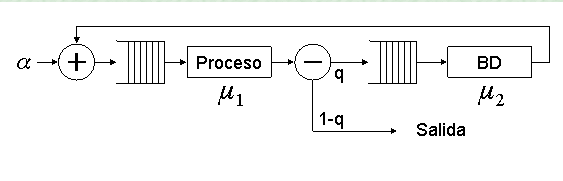
\includegraphics[keepaspectratio=true,width=\linewidth]{img/ej15.png}
\end{center}

Las transacciones emplean un tiempo de proceso distribuido exponencialmente con media $1/μ_1$. Tras este tiempo, la ejecución del programa se completa con una probabilidad 1-q, o requiere acceder a un servidor de base de datos y continuar su proceso. Suponer que la recuperación de la información de la base de datos requiere un tiempo distribuido exponencialmente con media $1/μ_2$.
\begin{enumerate}
\item Justificar adecuadamente los modelos de colas que se deben emplear para modelizar el sistema.
\item Calcular el tiempo medio de estancia en el sistema de las peticiones de los clientes.
\end{enumerate}
\TheSolution

\begin{enumerate}
\item Se trata de una red de colas donde cada cola sigue un modelo M/M/1

\item

Primero tenemos que calcular las tasas de llegadas:
\[λ_1 = α+qλ \implies λ = \frac{α}{1-q}\]
\[λ_2 = q λ_1\]

Ahora podemos calcular el factor de utilización de cada uno de los subsistemas:
\[ρ_1 = \frac{λ_1}{μ_1} = \frac{α}{μ_1(1-q)}\]
\[ρ_2 = \frac{λ_2}{μ_2} = \frac{q\cdot α}{μ_2(1-q)}\]

A partir de estos valores calculamos $L_1$ y $L_2$ y por último calculamos el tiempo medio de estancia en el sistema como:
\[W = \frac{\sum L_i}{\sum α_i}=\frac{L_1+L_2}{α}\]

Puesto que no tenemos datos numéricos no terminamos de realizar las cuentas, pues no aportarán información nueva.
\end{enumerate}

%%%%%%%%%%%%%%%%%%%%%%%%%%%%%%%%%%%%%%%%%%%%%%%%%%%%%%%%%%%%%%%%%%%%%%%%%% PROBLEMA 16

\Problem
El tiempo que emplea un determinado servidor de control de accesos de una red en procesar una solicitud de autenticación de un usuario se puede considerar como una variable aleatoria con distribución exponencial de valor esperado 235 ms. Debido a su construcción, tiene una cola de espera limitada, de modo que rechaza cualquier nueva solicitud que reciba cuando ya se encuentra procesando una y hay otras dos en espera. Si se supone que el número de clientes del servidor es muy grande, y que las peticiones que realizan siguen un ritmo de Poisson con una tasa de 5 peticiones por segundo, calcular la probabilidad de que se rechace una solicitud, la ocupación media del servidor y el tiempo medio de estancia en el sistema de las peticiones que son procesadas

\TheSolution

Estamos ante un modelo M/M/1/K siendo $K=3$. Tenemos la tasa de llegadas $λ=5$ y la tasa de servicio $μ=1/T_s=4.25$.

La probabilidad de que se rechace una solicitud es la probabilidad de que haya tres o más clientes en el sistema:
\[\mathbb{P}(\text{rechazo}) = 1- p_1-p_2 = 1-p_0\frac{λ}{μ}-p_0\left( \frac{λ}{μ}\right)^2 = 1-\frac{1-λ/μ}{1-(λ/μ)^{4}}\frac{λ}{μ}-\frac{1-λ/μ}{1-(λ/μ)^{4}}\left( \frac{λ}{μ}\right)^2 = 0.5\]

La ocupación media del servidor se calcula con la fórmula:
\[L=\frac{λ/μ}{1-λ/μ}\frac{1-4(λ/μ)^3+3(λ/μ)^4}{1-(λ/μ)^4}=1.69\]

Para el tiempo medio de estnacia en el servidor aplicamos el teorema de Little con lo que obtenemos
\[W = \frac{L}{λ}=0.56s\]

%%%%%%%%%%%%%%%%%%%%%%%%%%%%%%%%%%%%%%%%%%%%%%%%%%%%%%%%%%%%%%%%%%%%%%%%%% PROBLEMA 17

\Problem En una instalación se tiene un problema con el tiempo de respuesta de un servidor de RPCs. El ordenador en el que reside dicho servicio tiene 2 CPUs dedicadas exclusivamente a procesar las peticiones, de modo que cualquiera de ellas puede atender cualquier petición en cualquier estado, y un sistema de disco único. El tráfico de llegada al servidor se puede suponer de Poisson, con un valor medio de R peticiones por segundo.

El proceso que se efectúa en el servidor necesita realizar un número variable de accesos a disco. Se ha estimado que cada petición emplea un tiempo de proceso en alguna de las CPUs que se encuentra distribuido exponencialmente con un valor medio T1. Transcurrido este periodo, la petición necesita acceder a disco con una probabilidad p, o finaliza en caso contrario.

El acceso al único disco del sistema emplea un tiempo distribuido exponencialmente, con un valor medio de T2.
Una vez realizado el acceso a disco, la petición volverá siempre a la cola de entrada en espera nuevamente de que alguna de las CPUs esté libre para continuar el proceso.

El tamaño de las colas de espera en cualquier parte del sistema se puede considerar infinito.

Datos numéricos: R = 2$s^{-1}$; p = 0.8; T1 = 20 ms.; T2 = 100 ms.
\begin{enumerate}
\item Dibujar el diagrama de bloques del sistema, indicando en él los puntos de encolamiento, tasas de peticiones recibidas en cada punto y tiempos de servicio de cada uno de los elementos que lo componen.
\item Calcular el número medio de unidades en cola en el sistema total.
\item Calcular el tiempo medio de estancia en el sistema de una petición.
\item A partir de los resultados obtenidos, identificar los ``cuellos de botella'' del sistema, y realizar sugerencias sobre las modificaciones que sería necesario introducir en el mismo para reducir el tiempo medio de estancia en él.
\end{enumerate}
\TheSolution

\begin{enumerate}
\item Se trata de una red de colas M/M/1

\item
El número medio de unidades en cola será la suma del número medio de unidades en cada una de las colas.

Las tasas de llegadas de cada cola son:
\[λ_1 = R + p \cdot λ_1 \implies λ_1 - p\cdot λ_1 = R \implies λ_1 = \frac{R}{1-p} = 10 s^{-1}\]
\[λ_2 = p\cdot R + p \cdot λ_2 \implies λ_2 - p\cdot λ_2 = p \cdot R \implies λ_2 = \frac{p\cdot R}{1-p} = p\cdot 10 s^{-1} = 8 s^{-1}\]

Conocemos ya los tiempos de servicio de cada ``subsistema'' de modo que podemos calcular las tasas de servicio:
\[μ_1 = \frac{1}{T_1/2}=100s^{-1}\]
\[μ_2 = \frac{1}{T_2}=10s^{-1}\]

Conocidos estos valores podemos calcular el factor de utilización de cada ``subsistema'' y con él el número medio de clientes en cada ``subsistema'':
\[ρ_1 = \frac{λ_1}{μ_1}=0.1 \implies L_1=\frac{ρ_1}{1-ρ_1} = 0.11\]
\[ρ_2 = \frac{λ_2}{μ_2}=0.8 \implies L_2=\frac{ρ_2}{1-ρ_2} = 4\]

Aplicando el teorema de Little podemos calcular el tiempo de estancia en cada ``subsistema'':
\[W_1 = \frac{L_1}{λ_1} = 0.011 s\]
\[W_2 = \frac{L_2}{λ_2} = 0.5 s\]

Sabiendo que el tiempo medio de estancia en el ``subsistema'' es la suma del tiempo medio de espera en cola más el tiempo medio de servicio, podemos calcular el tiempo medio de espera en cola de cada ``subsistema'' es que:
\[TC_1 = W_1-T1/2 = 1 ms = 0.001 s\]
\[TC_2 = W_2-T2 = 400 ms = 0.4s\]

Aplicando nuevamente el teorema de little podemos calcular el número medio de clientes en cada cola:
\[Lq_1 = λ_1TC_1 = 0.01\]
\[Lq_2 = λ_2TC_2 = 3.2\]

El número medio de clientes en cola en el sistema total será la suma del número medio de clientes en cada una de las colas, es decir, tenemos que
\[Lq = Lq_1+Lq_2 = 3.21 \text{clientes}\]

\item

El tiempo medio de estancia en el sistema de una petición se calcula de la siguiente forma:
\[W = \frac{\sum L_i}{\sum α_i}=2.06s\]

También podríamos calcularlo como:
\[W = W_1+pW_2+pW \implies W = \frac{W_1+pW_2}{1-p}=2.06s\]

Estamos teniendo en cuenta el hecho de que no todas las peticiones pasan por ambos ``subsistemas'' al multiplicar por $p$.

Por otro lado estamos considerando la recursividad a la hora de calcular la tasa de llegadas a cada uno de los ``subsistemas'', dato en que nos hemos basado para calcular los tiempos medios de estancia.

\item

A partir de estos datos podemos observar que el cuello de botella en el sistema es el acceso al disco que, por ser disco único y tener tiempo de acceso 5 veces mayor que el tiempo de procesamiento en cada una de las 2 CPUs, lleva 10 veces más tiempo que el procesamiendo de la petición.

Habría que disminuir este tiempo mediante una sustitución del disco por uno más rápido, permitiendo múltiples accesos simultáenos al disco o aumentando el número de discos.

\end{enumerate}

%%%%%%%%%%%%%%%%%%%%%%%%%%%%%%%%%%%%%%%%%%%%%%%%%%%%%%%%%%%%%%%%%%%%%%%%%% PROBLEMA 18
\Problem
Se ha detectado que el cuello de botella en una aplicación se produce al leer del disco. Para solucionarlo, se plantean dos alternativas:
\begin{itemize}
\item Comprar un disco con tiempo de acceso menor, pero más caro. En este caso, se encolan las peticiones cuando el disco se encuentre ocupado.
\item Poner dos discos en espejo (mirroring) que tendrán un tiempo de acceso mayor que el anterior, pero más baratos. En este caso, se accede indistintamente a cualquiera de los dos discos cuando se produce una petición, dependiendo de cuál esté libre, encolándose todas las peticiones en una cola común.
\end{itemize}
(Datos numéricos: tiempo medio de acceso disco rápido: 10 ms; tiempo medio de acceso de cada disco lento: 15 ms. En ambos casos se supone distribución exponencial).

Suponiendo que la aplicación es la única que realiza los accesos a disco, que las peticiones de lectura se producen según un proceso de Poisson, y que las colas se pueden suponer infinitas:
\begin{enumerate}
\item Calcular para ambos casos el número medio de peticiones por segundo que se podrán satisfacer para obtener un tiempo medio de lectura igual a 100 ms.
\item Calcule la tasa de peticiones para la que ambos casos dan el mismo rendimiento, y el tiempo medio de lectura para este caso.
\end{enumerate}

\TheSolution

\textcolor{red}{Por hacer}

%%%%%%%%%%%%%%%%%%%%%%%%%%%%%%%%%%%%%%%%%%%%%%%%%%%%%%%%%%%%%%%%%%%%%%%%%% PROBLEMA 19
\Problem
Un servidor de validación de firmas que se encuentra en una determinada red procesa mensajes de modo iterativo. Los mensajes de solicitud que recibe tienen un tamaño medio de 100 bytes, y se puede suponer que su llegada al servidor sigue un proceso de Poisson. El tiempo de proceso de cada mensaje es aleatorio, sabiéndose que su valor medio es 10 ms. y que su distribución de probabilidades se puede considerar exponencial.

La monitorización de la red únicamente nos permite conocer el tamaño medio de la ocupación que tiene en memoria la cola donde se almacenan los mensajes pendientes de procesar, que es de 325 bytes.
\begin{enumerate}
\item Calcular el tiempo medio total que transcurre desde que llega un mensaje de petición al servidor y este termina de procesarlo.
\item En los acuerdos de nivel de servicio de este servidor se establece que ``El tiempo que debe transcurrir desde que llegue un mensaje de petición al servidor y este termine de procesarlo debe ser inferior a 80 ms en el 90\% de las peticiones''. Explicar razonadamente si se cumple o no este punto del acuerdo de nivel de servicio. En caso negativo, sugerir cualitativamente soluciones que permitirían resolver el problema.
\end{enumerate}

\TheSolution

\textcolor{red}{Por hacer}

%%%%%%%%%%%%%%%%%%%%%%%%%%%%%%%%%%%%%%%%%%%%%%%%%%%%%%%%%%%%%%%%%%%%%%%%%% PROBLEMA 20

%%%%%%%%%%%%%%%%%%%%%%%%%%%%%%%%%%%%%%%%%%%%%%%%%%%%%%%%%%%%%%%%%%%%%%%%%% PROBLEMA 21
\Problem[21] Un determinado bufete de abogados tiene, entre otras actividades, un servicio de generación de informes legales sobre los asuntos que sus clientes le plantean. Para ayudar al personal del bufete en la gestión de dicho servicio se dispone de un sistema de gestión de flujo de trabajo.

El flujo de trabajo que siguen las peticiones recibidas es el siguiente:
\begin{enumerate}
\item[1] Un primer empleado, que denominaremos E1, verifica que las peticiones son correctas, recopila información asociada a ellas y las clasifica para su posterior proceso en dos grupos distintos: civil o penal. Se reciben en promedio un 25 \% de peticiones de tipo penal y un 75 \% de tipo civil. Este proceso de revisión, acopio de información y clasificación se realiza en un tiempo medio de 1 día. Cada grupo de peticiones es enviado, a través del sistema de gestión de flujo de trabajo, a un grupo de empleados distintos.

\item[2] Las peticiones de tipo civil son recibidas por el empleado C1, que es el encargado de elaborar el informe. Este empleado tarda un tiempo medio de 4 días en realizar un informe. Tras la realización del informe, el empleado C2 revisa el trabajo del primero, determinando si el informe es correcto, y puede seguir su curso, o si necesita un trabajo posterior, en cuyo caso lo devuelve anotado a la bandeja de entrada de C1 para que realice las correcciones oportunas. C2 emplea un tiempo medio de 2 días en realizar esta revisión, y se sabe que, en promedio, la mitad de los informes que recibe C2 necesitan volver a C1 para ser modificados.

\item[3] Las peticiones de tipo penal siguen un proceso idéntico a las de tipo civil, pero las realizan los empleados P1 y P2. P1 emplea en el primer proceso un tiempo medio de 10 días por petición, mientras que P2 emplea solamente 4 días. El porcentaje promedio de documentos que son devueltos a P1 es de un 25 \%.

\item[4] Tras ser aceptado un informe de cualquiera de los dos grupos, pasa al departamento de acabado final, donde el empleado E2 realiza su impresión en calidad, encuadernado y envío al cliente que lo solicitó. En este proceso se emplean 0.25 días.
\end{enumerate}

En la empresa se recibe un promedio de una petición cada D días laborables.
El sistema de flujo de trabajo realiza el encolamiento de las solicitudes y los informes elaborados en su paso a través del proceso establecido.

Para realizar los cálculos que se piden a continuación, suponer que todos los tiempos indicados son variables aleatorias distribuidas exponencialmente.
\begin{enumerate}
\item Dibujar el esquema del sistema de control de flujo de trabajo establecido, visto como una red de colas, en la que cada empleado es el servidor que procesa las peticiones recibidas. Calcular las tasas de servicio de cada uno de los servidores, y las tasas de peticiones que recibe cada uno de ellos, indicando las suposiciones que haya sido necesario realizar para poder obtener dichos valores.
\item Calcular el tiempo medio que tarda el bufete en realizar un informe desde que es recibida la solicitud del cliente.
\end{enumerate}

\TheSolution
\begin{enumerate}
\item


A la hora de realizar el esquema del sistema suponemos que las colas son infinitas puesto que un empleado puede tener una pila de trabajo pendiente tan grande como sea necesaria.

La tasa de servicio se calcula igual para todos los servidores, mediante la fórmula:
\[μ = \frac{1}{T_s}\]

La siguiente tabla recoge los resultados:


\begin{center}
\begin{tabular}{| c |  c |}
\hline
  \textbf{Servidor/Empleado}  & \textbf{Tasa de servicio (μ) [$s^{-1}$]}\\
\hline
 \textit{E1}& 0.000011574\\
 \textit{C1}& 0.000002894\\
 \textit{C2}& 0.000005787\\
 \textit{P1}& 0.000001157\\
 \textit{P2}& 0.000002894\\
 \textit{E2}& 0.000046296\\
\hline
\end{tabular}
\end{center}

La tasa de llegadas de cada servidor es:

\begin{center}
\begin{tabular}{| c |  c |}
\hline
  \textbf{Servidor/Empleado}  & \textbf{Tasa de llegadas (λ) [$s^{-1}$]}\\
\hline
 \textit{E1}& $1/D$\\
 \textit{C1}& $3/(2D)$\\
 \textit{C2}& $λ_{C_1} = 3/(2D)$\\
 \textit{P1}& $1/(3D)$\\
 \textit{P2}& $λ_{P_1} = 1/(3D)$\\
 \textit{E2}& $0.5 \cdot λ_{C_1}+0.75 \cdot λ_{P_1} = 1/D$\\
\hline
\end{tabular}
\end{center}

Para los servidores $C_1$ y $P_1$ hemos calculado la tasa de llegadas como sigue
\[λ_{C_1}=\frac{0.75}{D}+λ_{C_1}\cdot 0.5 \implies λ_{C_1} = \frac{0.75}{D \cdot 0.5} = \frac{3}{2\cdot D}\]
\[λ_{P_1}=\frac{0.25}{D}+λ_{P_1}\cdot 0.25 \implies λ_{P_1} = \frac{0.25}{D \cdot 0.75} = \frac{1}{D \cdot 3}\]

\item

Vamos a considerar los subsistemas de procesamiendo de peticiones civiles y penales de manera independiente, puesto que tienen retroalimentación, y calculamos su tiempo medio de servicio.

Con los datos que ya tenemos calculados, podemos conocer el factor de utilización y el número medio de clientes de cada uno de los servidores. A partir de este número, aplicamos el teorema de Little para obtener el tiempo medio de estancia en cada uno de estos servidores. Finalmente, para calcular el tiempo total sólo debemos sumar los tiempos ponderados.

La siguiente tabla recoge los valores calculados según acabamos de indicar:

\begin{adjustwidth}{-2cm}{-2cm}
\begin{center}
\begin{tabular}{| c | c | c | c |}
\hline
  \textbf{S/E}  & \textbf{ρ = λ/μ = λT} & \textbf{L  = ρ/(1-ρ) [clientes]} & \textbf{W  = L/λ  [s/cliente]}\\
\hline
 \textit{E1}& $1/D$ & $1/(D-1)$ & $D/(D-1)$ \\
 \textit{C1}& $6/D$ & $6/(D-6)$ & $4D/(D-6)$ \\
 \textit{C2}& $3/D$ & $3/(D-3)$ & $2D/(D-3)$ \\
 \textit{P1}& $10/(3D)$ & $10/(3D-10)$ & $30D/(3D-10)$ \\
 \textit{P2}& $4/(3D)$ & $4/(3D-4)$ & $12D/(3D-4)$ \\
 \textit{E2}& $1/(4D)$ & $1/(4D-1)$ & $D/(4D-1)$ \\
\hline
\end{tabular}
\end{center}
\end{adjustwidth}

Finalmente procedemos a calcular el tiempo medio de estancia en el sistema, que será el tiempo medio que tarde el bufete en realizar un informe:
%\[W = W_{E_1}+0.25(W_{P_1}+W_{P_2})+0.75(W_{C_1}+W_{C_2})+W_{E_2}\]
\[W = \frac{\sum L_i}{\sum α_i}=\frac{\sum L_i}{1/D}\]
\end{enumerate}

%%%%%%%%%%%%%%%%%%%%%%%%%%%%%%%%%%%%%%%
%%%%%%%%%%%%%%%%%%%%%%%%%%%%%%%%%%%%%%%
%%%%%%%%%%%%%%%%%%%%%%%%%%%%%%%%%%%%%%%

%%%%%%%%%%%%%%%%%%%%%%%%%%%%%%%%%%%%%%%%%%%%%%%%%%%%%%%%%%%%%%%%%%%%%%%%%% PROBLEMA 22
\Problem[22]
Se realizan medidas sobre el tiempo que emplea en procesar peticiones un servidor de aplicaciones, descubriendo que su distribución de probabilidades se puede aproximar por una función de Pareto de parámetros tm=5 ms y k=3. Partiendo de estos datos:

\begin{enumerate}
\item Si el servidor recibe un tráfico de Poisson con un valor medio de 100 peticiones/s, calcule el valor medio del tiempo de respuesta del servidor a las peticiones del usuario.

\item Si la salida del servidor de aplicaciones se recibe a la entrada de un servidor de registro de tráfico que tiene un tiempo de servicio distribuido exponencialmente, y que es capaz de procesar un promedio de 10000 peticiones/s, comentar qué modelo de sistema de colas sería adecuado para representar el comportamiento de este servidor. Escribir el modelo elegido en notación de Kendall.

\end{enumerate}

\textbf{Nota: } La función de densidad de una distribución de Pareto viene dada por la fórmula:
\[f(t)=k\frac{t_m ^k}{t^{k+1}} \text{ para } t > t_m\]

\TheSolution

\begin{enumerate}
\item Primero tenemos que calcular el tiempo medio de servicio. Para ello calculamos la esperanza de la distribución que nos dan:

\[T_s = \int 3t \frac{125}{t^4} = 1.8 ms\]

A partir de aquí podemos calcular la tasa de servicio
\[μ=\frac{1}{T_s}=559 s^{-1}\]

Calculamos ahora el factor de utilización y con él el número medio de clientes en el sistema, pues estamos ante un sistema M/M/1
\[ρ=\frac{λ}{μ}=0.18 \implies L= \frac{ρ}{1-ρ}=0.22\]

Con esto podemos calcular el tiempo medio de respuesta apoyándonos en el teorema de Little:
\[W = \frac{L}{λ} = 2.195\cdot 10^{-3}\]

\item

Deberíamos utilizar una red de colas con dos servidores M/M/1

\end{enumerate}

%%%%%%%%%%%%%%%%%%%%%%%%%%%%%%%%%%%%%%%%%%%%%%%%%%%%%%%%%%%%%%%%%%%%%%%%%% PROBLEMA 23
\Problem[23]
Un sistema de proceso de transacciones emplea un monitor de proceso de tipo híbrido. Mantiene una cola de llegada de solicitudes que son atendidas en cualquiera de los dos procesos que mantiene permanentemente activos para este fin. Las solicitudes de ejecución de transacciones llegan al sistema siguiendo un proceso de Poisson, con una tasa de llegadas de 50 peticiones / s. El tiempo de ejecución de una transacción es independiente del resto de los procesos que se encuentre ejecutando el sistema. Dicho tiempo se puede considerar distribuido exponencialmente, con un valor medio de 0.02 s.
\begin{enumerate}
\item Calcular el tiempo medio de estancia en el sistema de cada petición, justificando adecuadamente el modelo de cálculo elegido.
\item Un análisis más detallado del sistema nos permite medir la varianza del tiempo de ejecución de la transacción, que resulta ser de 0.00036. Justificar razonadamente la validez o no del modelo elegido en el caso anterior, proponiendo, en caso de que no sea válido, modelos alternativos de cálculo.
\end{enumerate}

\TheSolution

%%%%%%%%%%%%%%%%%%%%%%%%%%%%%%%%%%%%%%%%%%%%%%%%%%%%%%%%%%%%%%%%%%%%%%%%%% PROBLEMA 24
\Problem[24]
Un sistema de proceso de transacciones emplea un monitor de proceso de tipo simple, necesitando un proceso por cada transacción en ejecución. Por motivos de rendimiento del sistema, el máximo número de procesos que se le permite ejecutar simultáneamente es de 5. Las solicitudes de ejecución de transacciones llegan al sistema siguiendo un proceso de Poisson, con una tasa de llegadas de 100 peticiones / s. El tiempo de ejecución de una transacción es independiente del resto de los procesos que se encuentre ejecutando el sistema. Dicho tiempo se puede considerar distribuido exponencialmente, con un valor medio de 0.01 s.
\begin{enumerate}
\item Calcular la probabilidad de que se rechace una solicitud de transacción por no haber un proceso libre para ejecutarla, justificando adecuadamente el modelo de cálculo elegido.
\item Calcular el tiempo medio de estancia en el sistema de una petición.
\end{enumerate}
\TheSolution

%%%%%%%%%%%%%%%%%%%%%%%%%%%%%%%%%%%%%%%%%%%%%%%%%%%%%%%%%%%%%%%%%%%%%%%%%% PROBLEMA 25
\Problem[25]
Un sistema distribuido construido bajo el modelo J2EE consta de dos capas: la capa de servicio Web, compuesta por un servidor, y la capa de servidores de aplicaciones, que consta de dos elementos que procesan en paralelo. El reparto de peticiones desde el servidor web a los servidores de aplicaciones se realiza de manera aleatoria y no es necesario guardar datos de los usuarios entre una petición y la siguiente.

El servidor web tiene cola de peticiones finita. Admite un máximo de 6 peticiones, que se procesan en secuencia.
En los servidores de aplicaciones se puede considerar que no hay límite para el número de peticiones que admiten.
Se reciben las peticiones siguiendo un proceso de Poisson a un ritmo promedio de 200 peticiones por segundo. Los tiempos de servicio de los servidores de ambas capas se puede considerar que siguen una distribución exponencial, con valor medio de 3 ms en el caso del servidor web y 9 ms en cualquiera de los servidores de aplicaciones.

\begin{enumerate}
\item Dibujar el esquema del sistema propuesto, e identificar las tasas de entrada efectivas en cada una de las capas. (No las calcule en este apartado, sólo exprese las fórmulas básicas que las relacionan con la tasa de entradas total).
\item Calcular la fracción de peticiones que se rechazan del sistema.
\item Calcular el tiempo medio de respuesta para las peticiones que no son rechazadas del sistema.
\item Identificar las soluciones más eficaces para mejorar el tiempo medio de respuesta calculado anteriormente.
\end{enumerate}
\TheSolution

%%%%%%%%%%%%%%%%%%%%%%%%%%%%%%%%%%%%%%%%%%%%%%%%%%%%%%%%%%%%%%%%%%%%%%%%%% PROBLEMA 26
\Problem[26]
Una empresa dispone de un monitor de proceso de transacciones que controla el acceso a una base de datos. El monitor recibe solicitudes con una frecuencia media de dos veces por segundo según una distribución de Poisson. Si el monitor está atendiendo alguna petición, las solicitudes que lleguen esperan en una cola cuya capacidad máxima es de ocho solicitudes. Si la cola está llena, la solicitud es rechazada y debe ser enviada de nuevo por el ordenador cliente.
Desde que el monitor acepta una transacción hasta que la da por terminada, transcurre un tiempo distribuido exponencialmente cuya esperanza matemática es de 500 milisegundos.
\begin{enumerate}
\item¿Qué modelo, según la notación de Kendall, será aplicable a este sistema?
\item Calcular el tiempo medio de estancia en el sistema de las peticiones de autenticación de los clientes.
\item ¿Qué pasaría si se ampliase la cola del monitor para darle una capacidad ilimitada?
\end{enumerate}

\TheSolution

%%%%%%%%%%%%%%%%%%%%%%%%%%%%%%%%%%%%%%%%%%%%%%%%%%%%%%%%%%%%%%%%%%%%%%%%%% PROBLEMA 27
\Problem[27]
El proceso de generación de un ticket en el Ticket Granting Server de una determinada implementación de Kerberos requiere la ejecución en serie de dos procesos independientes:
Proceso A: valida el ticket de la solicitud recibida. Su tiempo de ejecución está distribuido exponencialmente, con valor medio de 98 ms. En promedio, se sabe que considera no válidos un 10\% de los tickets recibidos, de modo que no pasan al proceso B más que un 90\% del total.
Proceso B: genera un nuevo ticket para el servidor solicitado. Tiene un tiempo de ejecución distribuido exponencialmente, con valor medio de 80 ms.
Ambos procesos son independientes y con colas de espera suficientemente grandes, de modo que no se producen pérdidas de peticiones. Ambos ejecutan las peticiones de manera iterativa.

El servidor recibe peticiones de generación de tickets de acuerdo a un proceso de Poisson, con tasa media de llegadas de 10 peticiones / s.

\begin{enumerate}
\item Determinar el modelo de colas adecuado para cada uno de los sistemas, y calcular la expresión genérica del tiempo medio de estancia en el sistema, a partir de la función de distribución de probabilidad del modelo nacimiento-muerte.
\item Calcular el tiempo medio de estancia en el conjunto del sistema de las peticiones aceptadas por el primer servidor.
\item Detectar cuál es el cuello de botella de este sistema, y ajustar el valor medio del tiempo de servicio en él para eliminarlo, de modo que el tiempo de estancia en el sistema total se reparta por igual entre ambos procesos.
\end{enumerate}
%%%%%%%%%%%%%%%%%%%%%%%%%%%%%%%%%%%%%%%%%%%%%%%%%%%%%%%%%%%%%%%%%%%%%%%%%% PROBLEMA 28

\Problem[28]
Una empresa decide poner en alta disponibilidad su servidor de autenticación de usuarios de la manera más económica que sea posible. Para ello, duplica el servidor, y para lograr el balanceo de carga entre ambos servidores realiza un sencillo programa. Dicho programa se instala en un tercer servidor, cuya dirección IP será a la que accedan a los usuarios. El programa de balanceo no admite encolamiento de las peticiones que recibe de los clientes, de modo que si se encuentra procesando una de ellas, rechaza todas las peticiones adicionales que le lleguen.
\begin{enumerate}
\item Si el tiempo de proceso del balanceo se encuentra distribuido exponencialmente con un valor medio de 2 ms., y el servidor recibe peticiones siguiendo un tráfico de Poisson con un valor medio de 250 peticiones / s., calcular la probabilidad de que una petición que reciba sea rechazada.
\item Cada uno de los servidores de autenticación tiene un tiempo de servicio con una distribución uniforme entre 5 y 10 ms., y su cola de espera de peticiones no está limitada. Calcular el tiempo medio de estancia en el conjunto del sistema balanceador-servidor de autenticación de las peticiones no rechazadas.
\end{enumerate}
\TheSolution


\end{document}